\documentclass[aspectratio=169, 10pt]{beamer}

% ---------- Tema y colores ----------
\usetheme{default}
\usecolortheme{default}
\setbeamertemplate{navigation symbols}{}
\setbeamertemplate{footline}[frame number]
\setbeamertemplate{frametitle continuation}{}

\definecolor{StanfordRed}{RGB}{140,21,21}
\definecolor{StanfordGray}{RGB}{77,77,77}
\definecolor{LightGray}{RGB}{240,240,240}
\definecolor{AccentBlue}{RGB}{0,84,166}
\definecolor{AccentGreen}{RGB}{0,130,100}
\definecolor{UCMBlue}{RGB}{4, 171, 226}
\definecolor{UCMNavy}{RGB}{20, 65, 134}

\setbeamercolor{frametitle}{fg=white, bg=UCMBlue}
\setbeamercolor{title}{fg=white}
\setbeamercolor{author}{fg=white}
\setbeamercolor{institute}{fg=white!80}
\setbeamercolor{structure}{fg=UCMBlue}
\setbeamercolor{block title}{bg=UCMBlue!15!white, fg=UCMBlue}
\setbeamercolor{block body}{bg=LightGray}
\setbeamercolor{alerted text}{fg=UCMBlue}
\setbeamercolor{example text}{fg=UCMBlue}

\setbeamerfont{frametitle}{series=\bfseries, size=\large}
\setbeamerfont{title}{series=\bfseries, size=\LARGE}
\setbeamerfont{block title}{series=\bfseries}

% ---------- Paquetes ----------
\usepackage[utf8]{inputenc}
\usepackage[T1]{fontenc}
\usepackage[provide=*,spanish]{babel}

\usepackage{amsmath, amssymb, bm}
\usepackage{tikz}
\usepackage{pgfplots}
\pgfplotsset{compat=1.18}
\usetikzlibrary{arrows.meta, shapes.geometric, positioning, fit, calc,
                decorations.pathreplacing, backgrounds, shadows, patterns}
\usepackage{booktabs}
\usepackage{xcolor}
\usepackage{multicol}
\usepackage{tcolorbox}
\tcbuselibrary{skins, breakable}

% ---------- Comandos útiles ----------
\newcommand{\R}{\mathbb{R}}
\newcommand{\E}{\mathbb{E}}
\newcommand{\Var}{\operatorname{Var}}
\newcommand{\MSE}{\operatorname{MSE}}
\newcommand{\Bias}{\operatorname{Sesgo}}
\newcommand{\y}{\bm{y}}
\newcommand{\X}{\bm{X}}
\newcommand{\bbeta}{\bm{\beta}}

\newcommand{\formula}[1]{%
  \begin{tcolorbox}[colback=UCMBlue!8, colframe=UCMBlue, arc=4pt,
                    boxsep=2pt, left=6pt, right=6pt, top=3pt, bottom=3pt]
  #1
  \end{tcolorbox}
}

% ---------- Portada ----------
\title{\textbf{Machine Learning}}
\subtitle{MDS-211 Magister en Data Science}
\author{Sergio Hernández\\ shernandez@ucm.cl}
\institute{ \begin{tikzpicture}
    \clip [rounded corners=1cm] (0,0) rectangle (4,2);
    \node[anchor=south west, inner sep=0pt] at (0,0) 
        {\includegraphics[width=4cm, height=2cm]{figures/mindslab.png}};
\end{tikzpicture}
\\ \textbf{Universidad Católica del Maule}}
\date{}

% ============================================================
\begin{document}
% ============================================================

% --- Título ---
{
\setbeamertemplate{background}{
  \begin{tikzpicture}[remember picture, overlay]
    \fill[UCMBlue] (current page.south west) rectangle (current page.north east);
    \fill[UCMBlue!70!black, opacity=0.5]
      (current page.south west) -- ++(0,3) -- ++(18,0) -- cycle;
    \foreach \i in {1,...,40}{
      \fill[white, opacity=0.04]
        ({random()*17}, {random()*10}) circle ({random()*0.3});
    }
  \end{tikzpicture}
}
\begin{frame}[plain]
  \vspace{1.2cm}
  \titlepage
  \begin{tikzpicture}[remember picture, overlay]
    \node[white, opacity=0.15, font=\fontsize{80}{80}\selectfont] 
      at (current page.east) [xshift=-2cm] {$\Sigma$};
  \end{tikzpicture}
\end{frame}
}

% --- Índice ---
\begin{frame}{Contenido}
  \begin{columns}[T]
  \column{0.48\textwidth}
  \tableofcontents[sections={1-4}]
  \column{0.48\textwidth}
  \tableofcontents[sections={5-8}]
  \end{columns}
\end{frame}

% ============================================================
\section{Motivación}
% ============================================================

\begin{frame}{ML Hype}
\begin{figure}
\includegraphics[scale=0.3]{figures/hype.png}
\end{figure}
\end{frame}

% ============================================================
\section{¿Qué es el Aprendizaje Estadístico?}
% ============================================================

\begin{frame}{¿Qué es el Aprendizaje Estadístico?}
\begin{columns}[T]
\column{0.52\textwidth}
  \vspace{0.2cm}
  Supongamos que observamos una \alert{respuesta} $Y$ y $p$
  \alert{predictores} $X_1, X_2, \ldots, X_p$.

  \vspace{0.3cm}
  Se asume que existe una relación:
  \formula{
    \centering $Y = f(X) + \varepsilon$
  }

  \vspace{0.2cm}
  \begin{itemize}
    \item $f$ es una función \textbf{desconocida} de $X = (X_1,\ldots,X_p)$
    \item $\varepsilon$ es el \textbf{error aleatorio irreducible}, 
          independiente de $X$ con $\E[\varepsilon]=0$
  \end{itemize}

  \vspace{0.3cm}
  \textbf{El Aprendizaje Estadístico} es el conjunto de métodos para
  \alert{estimar} $f$.

\column{0.45\textwidth}
  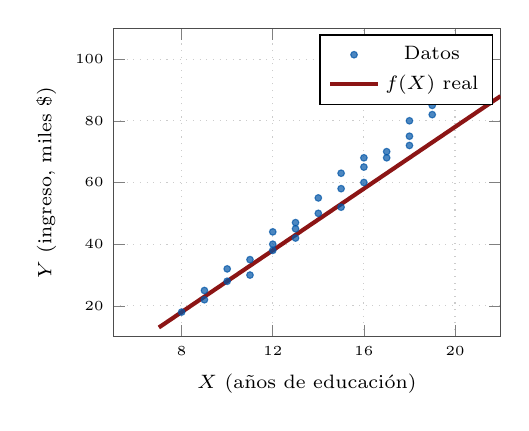
\begin{tikzpicture}
    \begin{axis}[
      width=6.5cm, height=5.5cm,
      xlabel={$X$ (años de educación)},
      ylabel={$Y$ (ingreso, miles \$)},
      xmin=5, xmax=22,
      ymin=10, ymax=110,
      xtick={8,12,16,20},
      ytick={20,40,60,80,100},
      tick label style={font=\tiny},
      label style={font=\scriptsize},
      grid=major, grid style={dotted, gray!40},
      axis line style={StanfordGray},
    ]
    % Scatter
    \addplot[only marks, mark=*, mark size=1.2pt,
             AccentBlue, opacity=0.7] coordinates {
      (8,18)(9,22)(10,28)(10,32)(11,30)(11,35)(12,40)(12,38)
      (13,42)(13,45)(14,50)(14,55)(15,58)(15,52)(16,60)(16,65)
      (17,70)(17,68)(18,75)(18,80)(19,82)(19,85)(20,88)(20,92)
      (21,95)(21,98)(9,25)(12,44)(15,63)(18,72)(16,68)(13,47)
    };
    % True f
    \addplot[domain=7:22, samples=80, 
             StanfordRed, thick, line width=1.5pt] 
      {5*x - 22};
    \legend{\scriptsize Datos, \scriptsize $f(X)$ real}
    \end{axis}
  \end{tikzpicture}
  \texttt{The Elements of Statistical Learning: Data Mining, Inference, and Prediction.
Trevor Hastie, Robert Tibshirani, Jerome H. Friedman. Springer Science \& Business Media, 2001
}
\end{columns}

\end{frame}

\begin{frame}{¿Por qué Estimar $f$?}
  \begin{columns}[T]
  \column{0.48\textwidth}
    \begin{block}{\textbf{Predicción}}
      \small
      Con una estimación $\hat{f}$, podemos predecir $Y$ para nuevas
      observaciones $X$:
      \[\hat{Y} = \hat{f}(X)\]
      El error cuadrático esperado descomponible es:
      \[
        \E\bigl[Y - \hat{Y}\bigr]^2 = 
        \underbrace{\bigl[f(X) - \hat{f}(X)\bigr]^2}_{\text{Reducible}} 
        + \underbrace{\Var(\varepsilon)}_{\text{Irreducible}}
      \]
      \vspace{0.2cm}
      $\Rightarrow$ Podemos minimizar solo el error \alert{reducible}.
    \end{block}
  \column{0.48\textwidth}
    \begin{block}{\textbf{Inferencia}}
      \small
      Comprender \textbf{cómo} $Y$ se relaciona con $X_1, \ldots, X_p$:
      \begin{itemize}
        \item ¿Qué predictores están \alert{asociados} con la respuesta?
        \item ¿Cuál es la \alert{dirección} de la relación?
        \item ¿La relación es \alert{lineal} o más compleja?
      \end{itemize}
    \end{block}

    \vspace{0.3cm}
    \begin{tcolorbox}[colback=AccentBlue!10, colframe=AccentBlue, arc=4pt,
                      boxsep=1pt, left=5pt, right=5pt, top=3pt, bottom=3pt]
      \small\textbf{Nota:} Predicción e Inferencia requieren diferentes
      métodos (interpretabilidad vs.\ precisión).
    \end{tcolorbox}
  \end{columns}
\end{frame}

% ============================================================
\section{Estimación de $f$}
% ============================================================

\begin{frame}{¿Cómo Estimamos $f$?}
\begin{columns}[T]
\column{0.50\textwidth}
  \vspace{0.2cm}
  \textbf{Datos de entrenamiento:}
  $\{(x_1, y_1), (x_2, y_2), \ldots, (x_n, y_n)\}$

  \vspace{0.2cm}
  Dos enfoques principales:

  \vspace{0.1cm}
  \begin{block}{\textbf{1. Métodos Paramétricos}}
    \small
    \begin{enumerate}
      \item Asumir una \textbf{forma funcional} para $f$\\
        Ej: $f(X) = \beta_0 + \beta_1 X$
      \item \textbf{Estimar los parámetros} a partir de datos\\
        Ej: mínimos cuadrados
    \end{enumerate}
    \textcolor{AccentGreen}{\small $\checkmark$ Simples} \quad
    \textcolor{StanfordRed}{\small $\times$ Pueden alejarse de la $f$ real}
  \end{block}

  \vspace{0.1cm}
  \begin{block}{\textbf{2. Métodos No Paramétricos}}
    \small
    No asumen forma para $f$; buscan una estimación
    \textbf{suave} que se ajuste a los datos.\\[4pt]
    \textcolor{AccentGreen}{\small $\checkmark$ Flexibles} \quad
    \textcolor{StanfordRed}{\small $\times$ Necesitan más datos ($n$ grande)}
  \end{block}

\column{0.48\textwidth}
  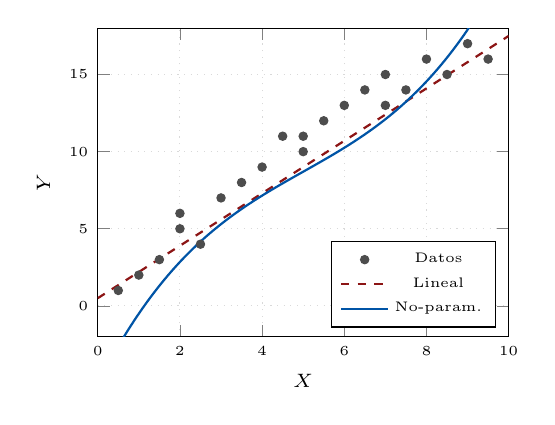
\begin{tikzpicture}
    \begin{axis}[
      width=6.8cm, height=5.5cm,
      xlabel={$X$}, ylabel={$Y$},
      xmin=0, xmax=10, ymin=-2, ymax=18,
      tick label style={font=\tiny},
      label style={font=\scriptsize},
      grid=major, grid style={dotted,gray!30},
      legend style={font=\tiny, at={(0.97,0.03)}, anchor=south east},
    ]
    \addplot[only marks, mark=*, mark size=1.5pt, StanfordGray] coordinates {
      (1,2)(1.5,3)(2,5)(2.5,4)(3,7)(3.5,8)(4,9)(4.5,11)
      (5,10)(5.5,12)(6,13)(6.5,14)(7,15)(7.5,14)(8,16)
      (8.5,15)(9,17)(9.5,16)(0.5,1)(2,6)(5,11)(7,13)
    };
    % Lineal
    \addplot[domain=0:10, StanfordRed, thick, dashed] {1.7*x + 0.5};
    % No paramétrico (spline simulado)
    \addplot[domain=0:10, samples=100, AccentBlue, thick] 
      {0.05*(x-5)^3 + 1.5*x + 1.2};
    \legend{Datos, Lineal, No-param.}
    \end{axis}
  \end{tikzpicture}
\end{columns}
\end{frame}

% ============================================================
\section{Compensación Sesgo–Varianza}
% ============================================================

\begin{frame}{Compensación Sesgo–Varianza}
\begin{columns}[T]
\column{0.52\textwidth}
  \vspace{0.1cm}
  El error de prueba esperado para un punto $x_0$ se descompone:

  \formula{
    \scriptsize
    \[\E\bigl[y_0 - \hat{f}(x_0)\bigr]^2 =
      \underbrace{\Var\!\bigl(\hat{f}(x_0)\bigr)}_{\text{Varianza}} +
      \underbrace{\bigl[\Bias\bigl(\hat{f}(x_0)\bigr)\bigr]^2}_{\text{Sesgo}^2} +
      \underbrace{\Var(\varepsilon)}_{\text{Irreducible}}\]
  }

  \vspace{0.3cm}
  \begin{itemize}
    \item \textbf{Varianza}: cuánto cambia $\hat{f}$ si usamos otro conjunto de entrenamiento
    \item \textbf{Sesgo}: error introducido al aproximar un problema real complejo con un modelo simple
  \end{itemize}

  \vspace{0.2cm}
  \alert{$\Rightarrow$ Más flexibilidad $\Rightarrow$ menos sesgo, más varianza}

\column{0.45\textwidth}
  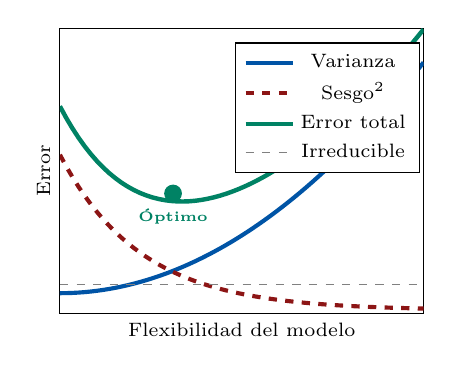
\begin{tikzpicture}
    \begin{axis}[
      width=6.2cm, height=5.2cm,
      xlabel={Flexibilidad del modelo},
      ylabel={Error},
      xmin=1, xmax=10, ymin=0, ymax=5,
      xtick=\empty, ytick=\empty,
      tick label style={font=\scriptsize},
      label style={font=\scriptsize},
      legend style={font=\scriptsize, at={(0.99,0.95)}, anchor=north east},
    ]
    % Varianza (sube con flexibilidad)
    \addplot[domain=1:10, samples=60, AccentBlue, thick, line width=1.5pt]
      {0.05*x^2 - 0.1*x + 0.4};
    % Sesgo^2 (baja con flexibilidad)
    \addplot[domain=1:10, samples=60, StanfordRed, thick, line width=1.5pt, dashed]
      {4.5*exp(-0.5*x) + 0.05};
    % Error total (U-shape)
    \addplot[domain=1:10, samples=60, AccentGreen, ultra thick]
      {0.05*x^2 - 0.1*x + 0.4 + 4.5*exp(-0.5*x) + 0.05 + 0.5};
    % Irreducible
    \addplot[domain=1:10, gray, dashed, thin] {0.5};
    \addplot[only marks, mark=*, mark size=3pt, AccentGreen] coordinates {(3.8, 2.1)};
    \node[font=\tiny, AccentGreen, anchor=north] at (axis cs:3.8,2.0) 
      {\textbf{Óptimo}};
    \legend{Varianza, Sesgo$^2$, Error total, Irreducible}
    \end{axis}
  \end{tikzpicture}
\end{columns}
\end{frame}

\begin{frame}{Sesgo–Varianza: Ilustración}
\centering
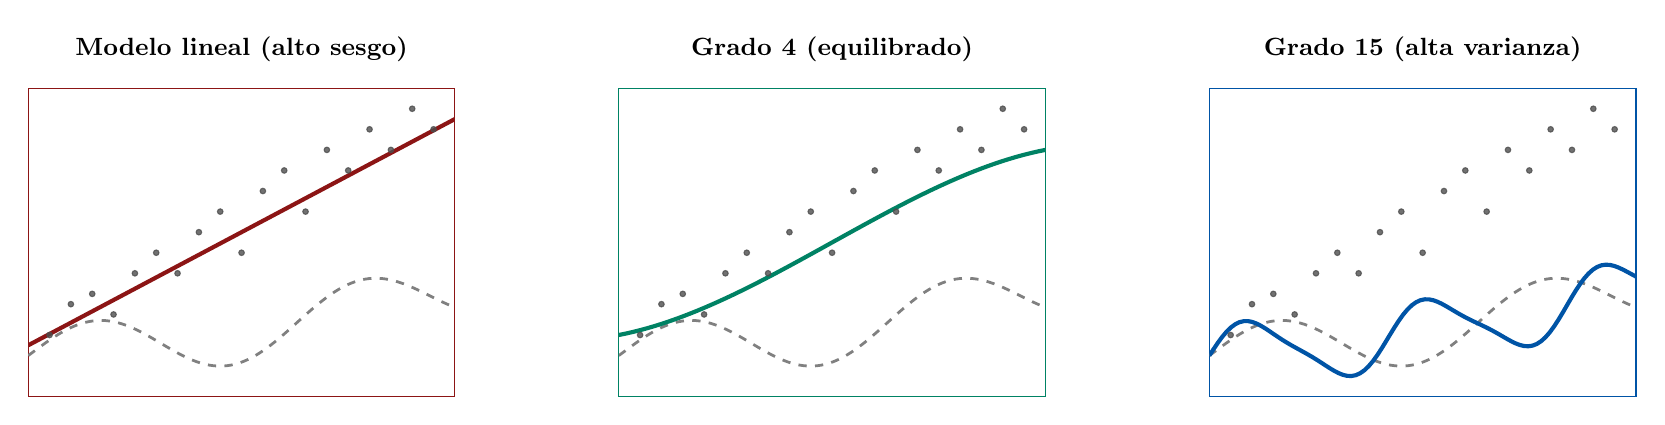
\begin{tikzpicture}
  % Three panels side by side
  \foreach \deg/\label/\xshift/\col in {
    1/{Modelo lineal (alto sesgo)}/0/StanfordRed,
    4/{Grado 4 (equilibrado)}/7.5/AccentGreen,
    15/{Grado 15 (alta varianza)}/15/AccentBlue}{
    \begin{scope}[xshift=\xshift cm]
      \begin{axis}[
        width=7cm, height=5.5cm,
        title={\small\textbf{\label}},
        title style={font=\footnotesize},
        xmin=0, xmax=10, ymin=-3, ymax=12,
        xtick=\empty, ytick=\empty,
        axis line style={\col},
        grid=major, grid style={dotted,gray!25},
        tick label style={font=\tiny},
        at={(0,0)},
      ]
      % True function
      \addplot[domain=0:10, samples=100, gray, thick, dashed, line width=1pt]
        {0.5*sin(deg(x))*3 + 0.1*x^1.5 - 1};
      % Scatter
      \addplot[only marks, mark=*, mark size=1pt, StanfordGray, opacity=0.8] 
        coordinates {
        (0.5,0)(1,1.5)(1.5,2)(2,1)(2.5,3)(3,4)(3.5,3)(4,5)
        (4.5,6)(5,4)(5.5,7)(6,8)(6.5,6)(7,9)(7.5,8)(8,10)(8.5,9)(9,11)(9.5,10)
      };
      % Fit line (just use polynomial approximations)
      \ifnum\deg=1
        \addplot[domain=0:10, \col, thick, line width=1.5pt]{1.1*x - 0.5};
      \fi
      \ifnum\deg=4
        \addplot[domain=0:10, samples=60, \col, thick, line width=1.5pt]
          {-0.01*x^3 + 0.15*x^2 + 0.4*x};
      \fi
      \ifnum\deg=15
        \addplot[domain=0:10, samples=100, \col, thick, line width=1.5pt]
          {0.5*sin(deg(1.5*x))*3 + 0.1*x^1.5 + 0.3*sin(deg(3*x)) - 1};
      \fi
      \end{axis}
    \end{scope}
  }
\end{tikzpicture}

\vspace{0.3cm}
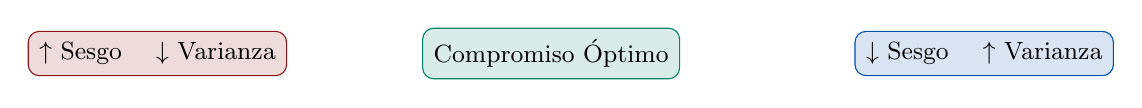
\begin{tikzpicture}
  \node[fill=StanfordRed!15, draw=StanfordRed, rounded corners, 
        inner sep=4pt, font=\small] 
    {$\uparrow$ Sesgo \quad $\downarrow$ Varianza};
  \node[fill=AccentGreen!15, draw=AccentGreen, rounded corners,
        inner sep=4pt, font=\small, xshift=5cm] 
    {Compromiso Óptimo};
  \node[fill=AccentBlue!15, draw=AccentBlue, rounded corners,
        inner sep=4pt, font=\small, xshift=10.5cm] 
    {$\downarrow$ Sesgo \quad $\uparrow$ Varianza};
\end{tikzpicture}
\end{frame}

% ============================================================
\section{Aprendizaje Supervisado vs.\ No Supervisado}
% ============================================================

\begin{frame}{Aprendizaje Supervisado vs.\ No Supervisado}
\begin{columns}[T]
\column{0.48\textwidth}
  \begin{block}{\textbf{Aprendizaje Supervisado}}
    \small
    Para cada observación $x_i$, existe una respuesta $y_i$ asociada.
    \begin{itemize}
      \item Regresión lineal, logística
      \item GAM, árboles, SVM, redes neuronales \ldots
    \end{itemize}
    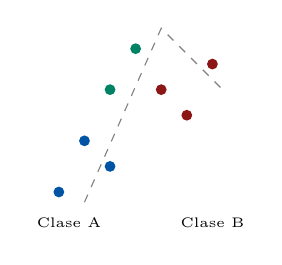
\begin{tikzpicture}[scale=0.65]
      \foreach \x/\y/\c in {
        1/1/AccentBlue, 1.5/2/AccentBlue, 2/1.5/AccentBlue,
        3/3/StanfordRed, 3.5/2.5/StanfordRed, 4/3.5/StanfordRed,
        2/3/AccentGreen, 2.5/3.8/AccentGreen}{
        \fill[\c] (\x,\y) circle (3pt);
      }
      \draw[gray,dashed] (1.5,0.8) -- (3,4.2) -- (4.2,3);
      \node[font=\tiny] at (1.2,0.4) {Clase A};
      \node[font=\tiny] at (4,0.4) {Clase B};
    \end{tikzpicture}
  \end{block}

\column{0.48\textwidth}
  \begin{block}{\textbf{Aprendizaje No Supervisado}}
    \small
    Solo se observan $x_i$; \textbf{no hay} respuesta $y_i$.
    Buscamos \alert{estructura oculta}.
    \begin{itemize}
      \item Análisis de clúster, PCA, mezclas gaussianas \ldots
    \end{itemize}
    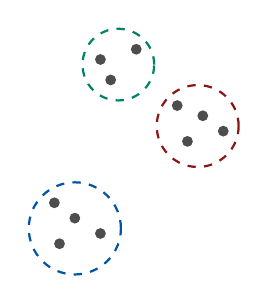
\begin{tikzpicture}[scale=0.65]
      \foreach \x/\y in {
        1/1, 1.3/1.5, 1.8/1.2, 0.9/1.8,
        3.5/3, 3.8/3.5, 4.2/3.2, 3.3/3.7,
        2/4.2, 2.5/4.8, 1.8/4.6}{
        \fill[StanfordGray] (\x,\y) circle (3pt);
      }
      \draw[AccentBlue, thick, dashed] (1.3,1.3) circle (0.9cm);
      \draw[StanfordRed, thick, dashed] (3.7,3.3) circle (0.8cm);
      \draw[AccentGreen, thick, dashed] (2.15,4.5) circle (0.7cm);
    \end{tikzpicture}
  \end{block}
\end{columns}
\end{frame}

% ============================================================
\section{Problemas de Regresión vs.\ Clasificación}
% ============================================================

\begin{frame}{Regresión vs.\ Clasificación}
\begin{columns}[T]
\column{0.48\textwidth}
  \begin{block}{\textbf{Regresión}}
    \small
    La respuesta $Y$ es \alert{cuantitativa} (numérica continua).
    \begin{itemize}
      \item Precio de una acción
      \item Temperatura máxima
      \item Ingreso anual
    \end{itemize}
    \vspace{0.2cm}
    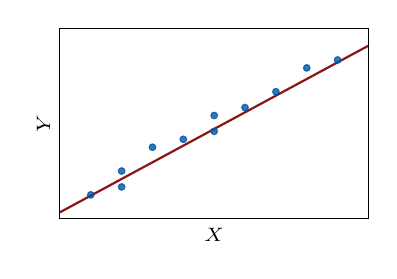
\begin{tikzpicture}
      \begin{axis}[
        width=5.5cm, height=4cm,
        xmin=0,xmax=10,ymin=0,ymax=12,
        xtick=\empty, ytick=\empty,
        xlabel={$X$}, ylabel={$Y$},
        label style={font=\scriptsize},
        grid=major, grid style={dotted,gray!30},
      ]
      \addplot[only marks, mark=*, mark size=1.2pt, AccentBlue, opacity=0.8]
        coordinates {
        (1,1.5)(2,3)(3,4.5)(4,5)(5,6.5)(6,7)(7,8)(8,9.5)(9,10)(2,2)(5,5.5)
      };
      \addplot[domain=0:10, StanfordRed, thick]{1.05*x+0.4};
      \end{axis}
    \end{tikzpicture}
  \end{block}

\column{0.48\textwidth}
  \begin{block}{\textbf{Clasificación}}
    \small
    La respuesta $Y$ es \alert{cualitativa} (categórica).
    \begin{itemize}
      \item Correo: ¿spam o no?
      \item Tumor: ¿maligno o benigno?
      \item Dígito manuscrito: 0--9
    \end{itemize}
    \vspace{0.2cm}
    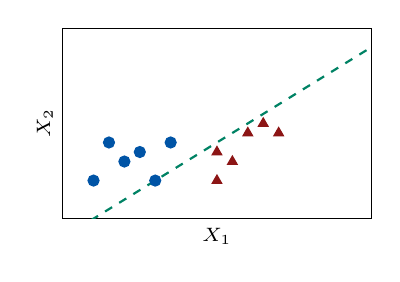
\begin{tikzpicture}
      \begin{axis}[
        width=5.5cm, height=4cm,
        xmin=0,xmax=10,ymin=0,ymax=10,
        xtick=\empty, ytick=\empty,
        xlabel={$X_1$}, ylabel={$X_2$},
        label style={font=\scriptsize},
        grid=major, grid style={dotted,gray!30},
      ]
      \addplot[only marks, mark=*, mark size=2pt, AccentBlue]
        coordinates {(1,2)(2,3)(1.5,4)(3,2)(2.5,3.5)(3.5,4)};
      \addplot[only marks, mark=triangle*, mark size=2pt, StanfordRed]
        coordinates {(5,2)(5.5,3)(5,3.5)(6,4.5)(6.5,5)(7,4.5)};
      \addplot[domain=0:10, AccentGreen, thick, dashed]{x-1};
      %\legend{\tiny Clase 1, \tiny Clase 2, \tiny Frontera}
      \end{axis}
    \end{tikzpicture}
  \end{block}
\end{columns}
\end{frame}

% ============================================================
\section{Evaluación de Modelos}
% ============================================================

\begin{frame}{Evaluación de la Calidad del Ajuste}
\begin{columns}[T]
\column{0.52\textwidth}
  \vspace{0.2cm}
  \textbf{Métrica más común — Regresión:}
  \formula{
    \centering
    $\displaystyle\MSE_{\text{entren.}} = 
    \frac{1}{n}\sum_{i=1}^n \bigl(y_i - \hat{f}(x_i)\bigr)^2$
  }

  \vspace{0.3cm}
  \begin{alertblock}{\small ¡El MSE de entrenamiento no es suficiente!}
    \small No nos interesa qué tan bien funciona el modelo en los
    datos que usamos para ajustarlo, sino en \textbf{datos nuevos}
    (datos de prueba).
  \end{alertblock}

  \vspace{0.3cm}
  \textbf{Queremos minimizar:}
  \formula{
    \centering
    $\displaystyle\MSE_{\text{prueba}} = 
    \E\bigl[(y_0 - \hat{f}(x_0))^2\bigr]$
  }

\column{0.45\textwidth}
  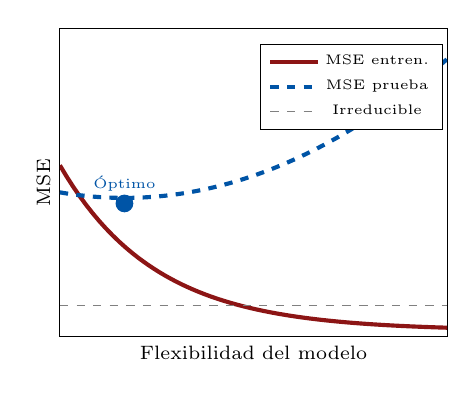
\begin{tikzpicture}
    \begin{axis}[
      width=6.5cm, height=5.5cm,
      xlabel={Flexibilidad del modelo},
      ylabel={MSE},
      xmin=1, xmax=10, ymin=0, ymax=5,
      xtick=\empty, ytick=\empty,
      label style={font=\scriptsize},
      legend style={font=\tiny, at={(0.99,0.95)}, anchor=north east},
      grid=major, grid style={dotted, gray!30},
    ]
    % MSE entrenamiento (decreasing)
    \addplot[domain=1:10, samples=60, StanfordRed, thick, line width=1.5pt]
      {4.2*exp(-0.45*x) + 0.1};
    % MSE prueba (U-shape)
    \addplot[domain=1:10, samples=60, AccentBlue, thick, line width=1.5pt, dashed]
      {0.04*x^2 - 0.2*x + 2.5};
    % Irreducible
    \addplot[domain=1:10, gray, dashed, thin] {0.5};
    % Optimal
    \addplot[only marks, mark=*, mark size=3pt, AccentBlue] 
      coordinates {(2.5, 2.16)};
    \node[font=\tiny, AccentBlue, anchor=south] at (axis cs:2.5, 2.2) {Óptimo};
    \legend{MSE entren., MSE prueba, Irreducible}
    \end{axis}
  \end{tikzpicture}
\end{columns}
\end{frame}

% ============================================================
\section{Sobreajuste}
% ============================================================

\begin{frame}{Sobreajuste (\textit{Overfitting})}
\begin{columns}[T]
\column{0.52\textwidth}
  \vspace{0.1cm}
  \begin{definition}
    Un modelo \alert{sobreajustado} aprende el \textbf{ruido} de los datos
    de entrenamiento, en lugar de la \textbf{señal} verdadera.
  \end{definition}

  \vspace{0.1cm}
  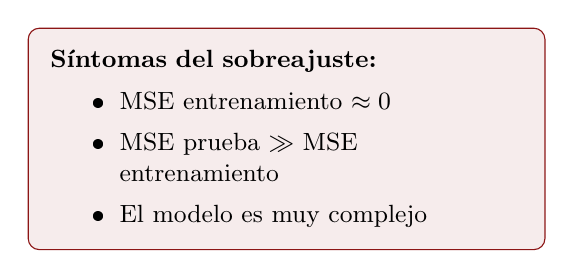
\begin{tikzpicture}
    \node[draw=StanfordRed, fill=StanfordRed!8, rounded corners,
          text width=6cm, align=left, inner sep=8pt, font=\small] {
      \textbf{Síntomas del sobreajuste:}
      \begin{itemize}
        \item MSE entrenamiento $\approx 0$
        \item MSE prueba $\gg$ MSE entrenamiento
        \item El modelo es muy complejo
      \end{itemize}
    };
  \end{tikzpicture}

  \vspace{0.1cm}
  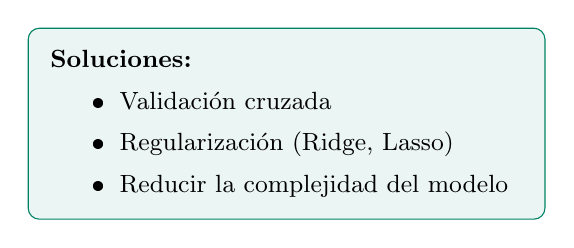
\begin{tikzpicture}
    \node[draw=AccentGreen, fill=AccentGreen!8, rounded corners,
          text width=6cm, align=left, inner sep=8pt, font=\small] {
      \textbf{Soluciones:}
      \begin{itemize}
        \item Validación cruzada
        \item Regularización (Ridge, Lasso)
        \item Reducir la complejidad del modelo
      \end{itemize}
    };
  \end{tikzpicture}

\column{0.45\textwidth}
  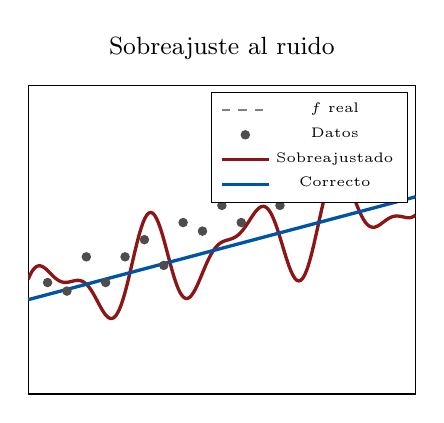
\begin{tikzpicture}
    \begin{axis}[
      width=6.5cm, height=5.5cm,
      title={\small Sobreajuste al ruido},
      xmin=0, xmax=10, ymin=-4, ymax=14,
      xtick=\empty, ytick=\empty,
      grid=major, grid style={dotted, gray!30},
      legend style={font=\tiny},
    ]
    % True f
    \addplot[domain=0:10, samples=100, gray, thick, dashed]{0.6*x + 1.5};
    % Noisy points
    \addplot[only marks, mark=*, mark size=1.5pt, StanfordGray] coordinates {
      (0.5,2.5)(1,2)(1.5,4)(2,2.5)(2.5,4)(3,5)(3.5,3.5)(4,6)(4.5,5.5)
      (5,7)(5.5,6)(6,8.5)(6.5,7)(7,9)(7.5,8.5)(8,10.5)(8.5,9.5)(9,11.5)
    };
    % Overfit (wiggly)
    \addplot[domain=0:10, samples=200, StanfordRed, thick, line width=1.2pt]
      {0.6*x + 1.5 + 2*sin(deg(2.5*x)) + 1.2*cos(deg(4*x))};
    % Good fit
    \addplot[domain=0:10, samples=60, AccentBlue, thick, line width=1.2pt]
      {0.6*x + 1.5};
    \legend{$f$ real, Datos, Sobreajustado, Correcto}
    \end{axis}
  \end{tikzpicture}
\end{columns}
\end{frame}

% ============================================================
\section{La Maldición de la Dimensionalidad}
% ============================================================

\begin{frame}{La Maldición de la Dimensionalidad}
\begin{columns}[T]
\column{0.52\textwidth}
  \vspace{0.1cm}
  Al aumentar $p$ (número de predictores):
  \begin{itemize}
    \item El volumen del espacio crece \textbf{exponencialmente}
    \item Los datos se vuelven \textbf{muy escasos}
    \item Los métodos locales (KNN) fallan
  \end{itemize}

  %\vspace{0.1cm}
  \begin{block}{Ejemplo}
    \small Para capturar el 10\% de los datos en $p$ dimensiones,
    necesitamos un vecindario que abarque:
    \[\ell = 0.1^{1/p}\]
    fracción del rango en cada dimensión.

    %\vspace{0.1cm}
    \begin{tabular}{cc}
      \toprule
      $p$ & $\ell$ \\
      \midrule
      1 & 10\% \\
      2 & 31.6\% \\
      10 & 79.4\% \\
      \bottomrule
    \end{tabular}
  \end{block}

\column{0.45\textwidth}
  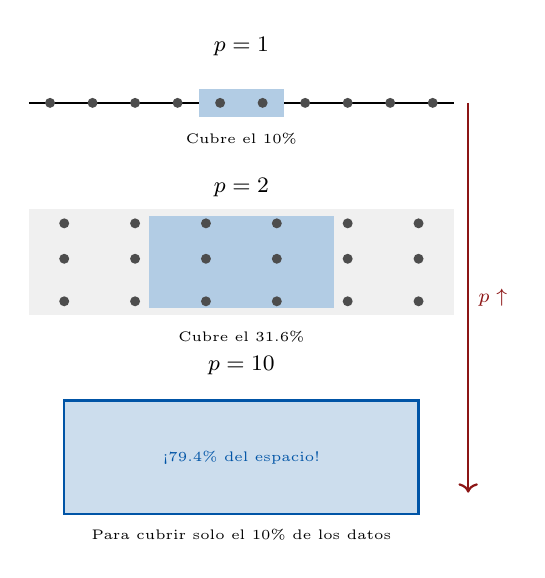
\begin{tikzpicture}[scale=0.9]
    % 1D
    \node[font=\footnotesize\bfseries] at (3, 6.8) {$p = 1$};
    \draw[thick] (0,6) -- (6,6);
    \fill[AccentBlue!30] (2.4,5.8) rectangle (3.6,6.2);
    \foreach \x in {0.3,0.9,1.5,2.1,2.7,3.3,3.9,4.5,5.1,5.7}
      \fill[StanfordGray] (\x,6) circle (2pt);
    \node[font=\tiny] at (3,5.5) {Cubre el 10\%};

    % 2D
    \node[font=\footnotesize\bfseries] at (3, 4.8) {$p = 2$};
    \fill[LightGray] (0,3) rectangle (6,4.5);
    \fill[AccentBlue!30] (1.7,3.1) rectangle (4.3,4.4);
    \foreach \x in {0.5,1.5,2.5,3.5,4.5,5.5}
      \foreach \y in {3.2,3.8,4.3}
        \fill[StanfordGray] (\x,\y) circle (2pt);
    \node[font=\tiny] at (3,2.7) {Cubre el 31.6\%};

    % 3D (simplified cube)
    \node[font=\footnotesize\bfseries] at (3, 2.3) {$p = 10$};
    \draw[fill=AccentBlue!20, draw=AccentBlue, thick] (0.5,0.2) rectangle (5.5,1.8);
    \node[font=\tiny, AccentBlue] at (3,1.0) {¡79.4\% del espacio!};
    \node[font=\tiny] at (3,-0.1) {Para cubrir solo el 10\% de los datos};

    % Arrow
    \draw[->, thick, StanfordRed] (6.2, 6) -- (6.2, 0.5) 
      node[midway, right, font=\scriptsize, StanfordRed] {$p \uparrow$};
  \end{tikzpicture}
\end{columns}
\end{frame}

% ============================================================
\section{Resumen y Modelos del Curso}
% ============================================================

\begin{frame}{Resumen: Conceptos Clave}
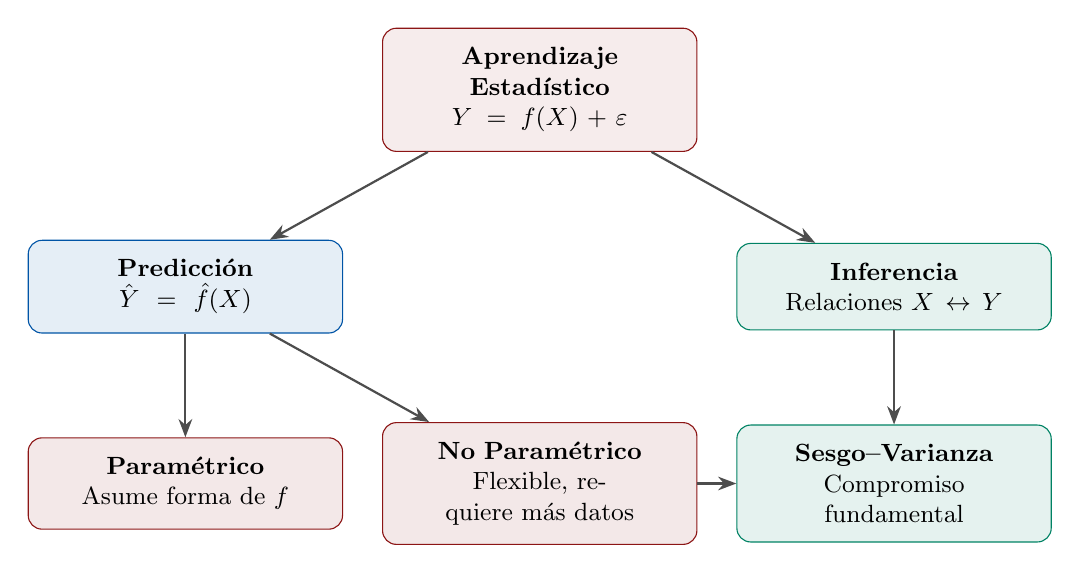
\begin{tikzpicture}[
  box/.style={draw=StanfordRed, fill=StanfordRed!8, rounded corners=5pt,
              text width=3.5cm, align=center, inner sep=7pt, font=\small},
  arrow/.style={->, >=Stealth, thick, StanfordGray},
]
  \node[box] (yl) at (0,0) 
    {\textbf{Aprendizaje Estadístico}\\ $Y = f(X) + \varepsilon$};
  \node[box, fill=AccentBlue!10, draw=AccentBlue] (pred) at (-4.5,-2.5) 
    {\textbf{Predicción}\\ $\hat{Y} = \hat{f}(X)$};
  \node[box, fill=AccentGreen!10, draw=AccentGreen] (inf) at (4.5,-2.5)
    {\textbf{Inferencia}\\ Relaciones $X \leftrightarrow Y$};
  \node[box, fill=StanfordRed!10, draw=StanfordRed] (param) at (-4.5,-5)
    {\textbf{Paramétrico}\\ Asume forma de $f$};
  \node[box, fill=StanfordRed!10, draw=StanfordRed] (nonparam) at (0,-5)
    {\textbf{No Paramétrico}\\ Flexible, requiere más datos};
  \node[box, fill=AccentGreen!10, draw=AccentGreen] (sv) at (4.5,-5)
    {\textbf{Sesgo–Varianza}\\ Compromiso fundamental};

  \draw[arrow] (yl) -- (pred);
  \draw[arrow] (yl) -- (inf);
  \draw[arrow] (pred) -- (param);
  \draw[arrow] (pred) -- (nonparam);
  \draw[arrow] (inf) -- (sv);
  \draw[arrow] (nonparam) -- (sv);
\end{tikzpicture}
\end{frame}



% --- Cierre ---


\end{document}